\begin{frame}[allowframebreaks]{Low-Rank Adaptation (LoRA)}
\begin{figure}
    \centering
    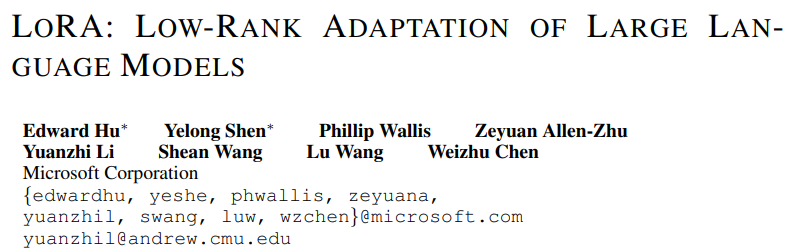
\includegraphics[width=\linewidth,height=0.72\textheight,keepaspectratio]{images/adv-img-gen/lora-1.png}
    \caption*{\scriptsize Source: Hu et al., \href{https://arxiv.org/abs/2106.09685}{``LoRA: Low-Rank Adaptation of Large Language Models''}, ICLR 2022.}
\end{figure}

\framebreak

\large \textbf{LoRA Overview}\\[0.5ex]
Low-Rank Adaptation (LoRA) is a technique for efficient fine-tuning of large neural networks. Instead of updating all parameters, LoRA injects trainable low-rank matrices into each layer, significantly reducing the number of trainable parameters.

\textbf{Key Idea:} Decompose the weight update $\Delta W$ as a product of two low-rank matrices:
\begin{equation}
    \Delta W = B A
\end{equation}
where $B \in \mathbb{R}^{d \times r}$ and $A \in \mathbb{R}^{r \times k}$, with $r \ll \min(d, k)$. Following Hu et al., $A$ is the down-projection (random Gaussian init) and $B$ the up-projection (initialised to zero), so $\Delta W = 0$ at the start of training.

\framebreak

\begin{figure}
    \centering
    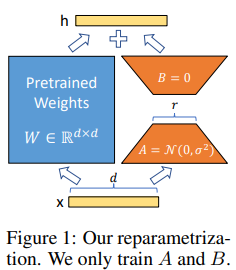
\includegraphics[width=\linewidth,height=0.72\textheight,keepaspectratio]{images/adv-img-gen/lora-2.png}
    \caption*{\scriptsize Source: Hu et al., \href{https://arxiv.org/abs/2106.09685}{``LoRA: Low-Rank Adaptation of Large Language Models''}, ICLR 2022.}
\end{figure}

\framebreak

\large \textbf{LoRA in Linear Layers}\\[0.5ex]
Consider a linear layer with weight $W_0 \in \mathbb{R}^{d \times k}$. In LoRA, the forward pass is modified as:
\begin{equation}
    y = W_0 x + \frac{\alpha}{r} B A x
\end{equation}
where $\alpha$ is a constant scaling factor and only $A$ and $B$ are updated during fine-tuning. Dividing by $r$ keeps the size of the update roughly independent of the rank, so $r$ can be changed without retuning the learning rate.

\textbf{Parameter Efficiency:} The number of trainable parameters is reduced from $d \times k$ to $r \times (d + k)$.

\framebreak
\large \textbf{LoRA Training Objective}\\[0.5ex]
The training objective remains the same as standard fine-tuning, e.g., minimizing a loss function $\mathcal{L}$:
\begin{equation}
    \min_{A, B} \mathcal{L}(\hat{y}, y)
\end{equation}
where $\hat{y}$ is the model output and $y$ is the ground truth.

\textbf{Regularization:} The rank bound is structural, not a penalty: $\Delta W = BA$ has rank at most $r$ by construction. Weight decay or dropout on the adapter branch can still be added to limit overfitting.

\framebreak
\large \textbf{LoRA in Attention Mechanisms}\\[0.5ex]
LoRA is commonly applied to the query and value projection matrices in attention layers:
\begin{align}
    W_q' &= W_q + \Delta W_q = W_q + \tfrac{\alpha}{r} B_q A_q \\
    W_v' &= W_v + \Delta W_v = W_v + \tfrac{\alpha}{r} B_v A_v
\end{align}
where $B_q, A_q, B_v, A_v$ are the low-rank factors for the query and value projections, respectively.

\framebreak

\begin{figure}
    \centering
    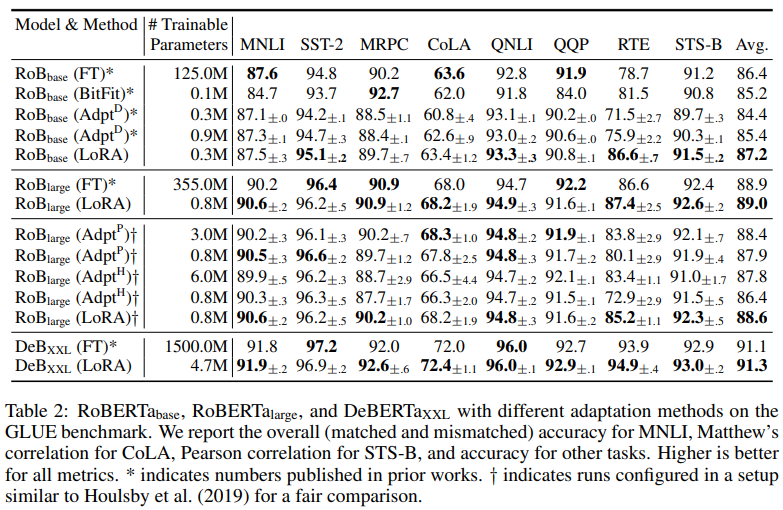
\includegraphics[width=\linewidth,height=0.72\textheight,keepaspectratio]{images/adv-img-gen/lora-3.png}
    \caption*{\scriptsize Source: Hu et al., \href{https://arxiv.org/abs/2106.09685}{``LoRA: Low-Rank Adaptation of Large Language Models''}, ICLR 2022.}
\end{figure}

\framebreak

\begin{figure}
    \centering
    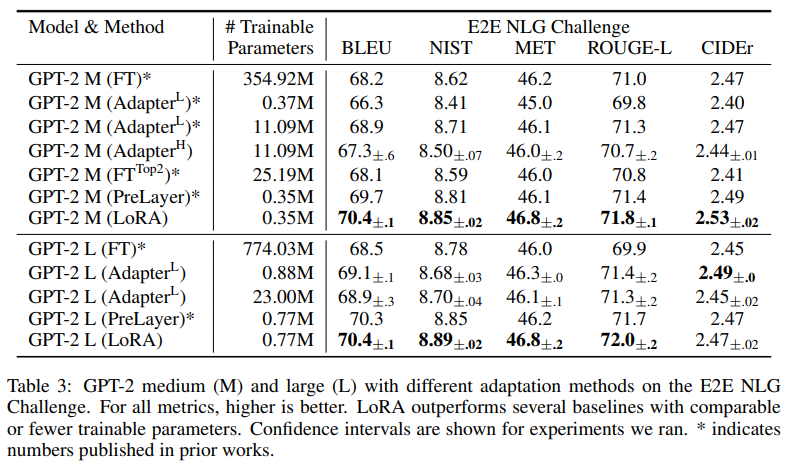
\includegraphics[width=\linewidth,height=0.72\textheight,keepaspectratio]{images/adv-img-gen/lora-4.png}
    \caption*{\scriptsize Source: Hu et al., \href{https://arxiv.org/abs/2106.09685}{``LoRA: Low-Rank Adaptation of Large Language Models''}, ICLR 2022.}
\end{figure}
\framebreak

\begin{figure}
    \centering
    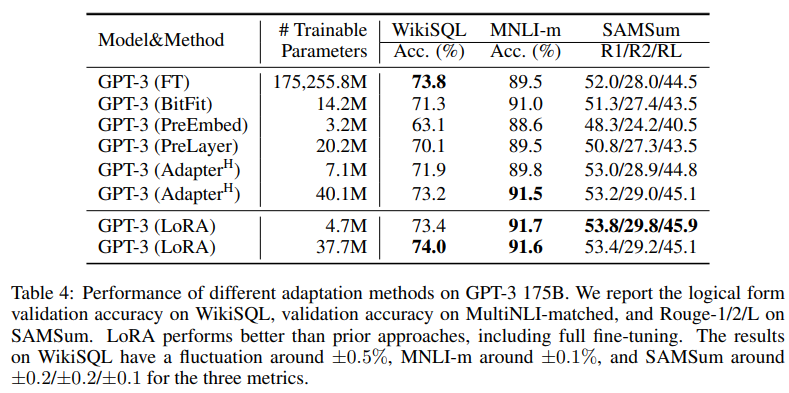
\includegraphics[width=\linewidth,height=0.72\textheight,keepaspectratio]{images/adv-img-gen/lora-5.png}
    \caption*{\scriptsize Source: Hu et al., \href{https://arxiv.org/abs/2106.09685}{``LoRA: Low-Rank Adaptation of Large Language Models''}, ICLR 2022.}
\end{figure}

\framebreak

\begin{figure}
    \centering
    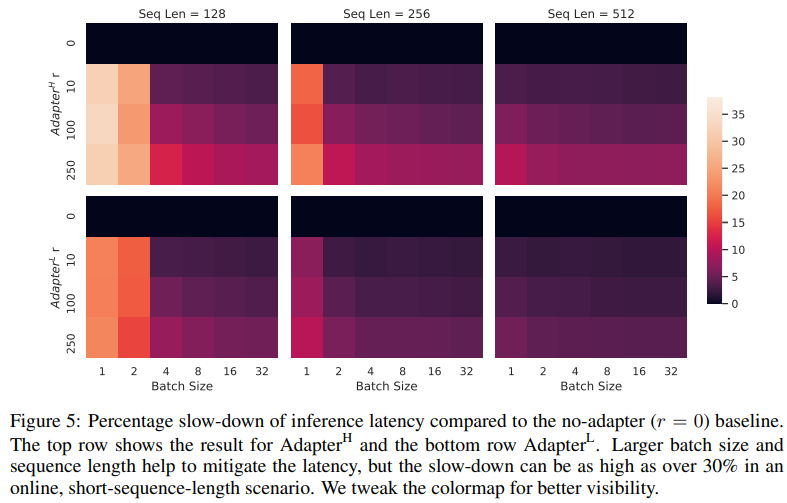
\includegraphics[width=\linewidth,height=0.72\textheight,keepaspectratio]{images/adv-img-gen/lora-6.png}
    \caption*{\scriptsize Source: Hu et al., \href{https://arxiv.org/abs/2106.09685}{``LoRA: Low-Rank Adaptation of Large Language Models''}, ICLR 2022.}
\end{figure}
\end{frame}